%% bare_jrnl.tex
%%%%%%%%%%%%%%%%%%%%%%%%%%%%%%%%%%%%%%%%%%%%%%%%
\documentclass[journal,12pt]{IEEEtran}
% Requires IEEEtran.cls in the same subdirectory
%%%%%%%%%%%%%%%%%%%%%%%%%%%%%%%%%%%%%%%%%%%%%%%%
\title{Barebones File for IEEE Journals}
\author{Michael~Shell,
        and~John~Doe% <-this % stops a space
\thanks{M. Shell and J. Doe are students with the Department of Information Technology, International College, Payap University, Chiang Mai 50000, Thailand}% <-this % stops a space
\thanks{This research paper is the report for an Unit assignment for IIT203 an undergraduate course in Discrete Mathematics taught by Dr. Robert P. Batzinger.}% <-this % stops a space
\thanks{Manuscript received  April 19, 2005; revised December 27, 2012.}}
\markboth{Journal of \LaTeX\ Class Files,~Vol.~11, No.~4, December~2012}%
{Shell and Doe: Bare Demo of IEEEtran.cls for Journals}
%%%%%%%%%%%%%%%%%%%%%%%%%%%%%%%%%%%%%%%%%%%%%%%%
% required packages
\usepackage{graphicx}
\usepackage[cmex10]{amsmath}
\usepackage{algorithm}
\usepackage{algorithmicx}
\usepackage{algpseudocode}
\usepackage{listings}
\usepackage{array}
\usepackage{url}
\usepackage{caption}
\usepackage{flushend}
\usepackage[dvipsnames]{xcolor}
%%%%%%%%%%%%%%%%%%%%%%%%%%%%%%%%%%%%%%%%%%%%%%%
% Document rendering options used
\bibliographystyle{IEEEtran}
\newtheorem{hyp}{H}
\captionsetup{justification=centering}
\lstset{% Style for Code segments
numbers=left,numberstyle=\tiny,
backgroundcolor=\color{yellow!15},
firstnumber=1, basicstyle=\footnotesize\ttfamily,
linewidth=\columnwidth,xleftmargin=20pt,
keywordstyle=\color{black}\bfseries,
identifierstyle=\color{MidnightBlue},
commentstyle=\color{Plum},
stringstyle=\color{OliveGreen},
showstringspaces=false,
breaklines=true,frame=lines,
numbersep=5pt
}
%%% Setup for Code Segments
\newcounter{cf}
\newfloat{code}{h}{cf}
\floatname{code}{Code Seg.}
\floatstyle{plaintop}
\restylefloat{code}
\hyphenation{op-tical net-works semi-conduc-tor}
%%%%%%%%%%%%%%%%%%%%%%%%%%%%%%%%%%%%%%%%%%%%%
\begin{document}
\maketitle

\begin{abstract}
The abstract goes here. The abstract should introduce the problem, mention a bit about the technology used and highlight the key findings, all within 150-250 words.
\end{abstract}

\begin{IEEEkeywords}
IEEEtran, journal, \LaTeX, paper, template.
\end{IEEEkeywords}

\section{Introduction}

\IEEEPARstart{T}{his} demo file is intended to serve as a ``starter file''
for IEEE journal papers produced under \LaTeX\ using
IEEEtran.cls version 1.8 and later. The first paragraph of the paper normally has a dropped letter and special font for the rest of the first word.
You must have at least 2 lines in the paragraph with the drop letter but this is not usually a problem. This section should contain the a basic overview of this research.\cite{Kopka:2003}

In general, published papers should be between 6,000 and 10,000 words. You need to say enough to make a logical case for your research without wasting words. 

\subsection{Description of the Problem}
The text of this subsection is to be included here. The first word is intended but rendered with a normal text font. This text unit is automatically numbered. This section provides background and description of the problem. 

\subsubsection{First Subsubsection}
Subsubsection text would go here. \LaTeXe\ will take care of the font changes, indentation, and numbering automatically. Replace the heading with the appropriate text.

\subsubsection{Second Subsubsection}
Subsubsection text would go here. \LaTeXe\ will take care of the font changes, indentation, and numbering automatically. Replace the heading with the appropriate text.

\begin{table}[htb]
\caption{A list of textbooks used for the course}
\label{textbookList}
\medskip
\centering
\small
\begin{tabular}{p{1.25in}rc}
\textbf{Author} & \textbf{Pages} & \textbf{Doc Type}\\
Code School\cite{CodeSchool:2013} & 20 & Ruby\\
Kopka\cite{Kopka:2003} & 559 & \LaTeX \\
Kwong\cite{Kwong:2015} & 307 & DisMath\\
Levin\cite{Levin:2017} & 345 & DisMath\\
Oetiker et als\cite{Oetiker:1996} & 63 & \LaTeX\\
Pine\cite{Pine:2014} & 216 & Ruby \\
Stein et als\cite{Stein:2011} & 526 & DisMath\\
Thomas\cite{Thomas:2013} & 863 & Ruby \\
\end{tabular}
\end{table}


\subsection{Research Strategy}
This subsection explains the rationale behind the direction used in the research to address this problem. I add a little more text here.

Clearly state the postulated or expected results of this work. Provide a listing of the hypothetical outcomes.

\begin{hyp}
The better the answer, the higher the score.
\end{hyp}

\begin{hyp}
The higher the score the better the grade
\end{hyp} 



A simple flowchart like that in Figure \ref{fig_flowchart} is a great way to illustrate the critical logic.

\begin{figure}[htb]
\centering
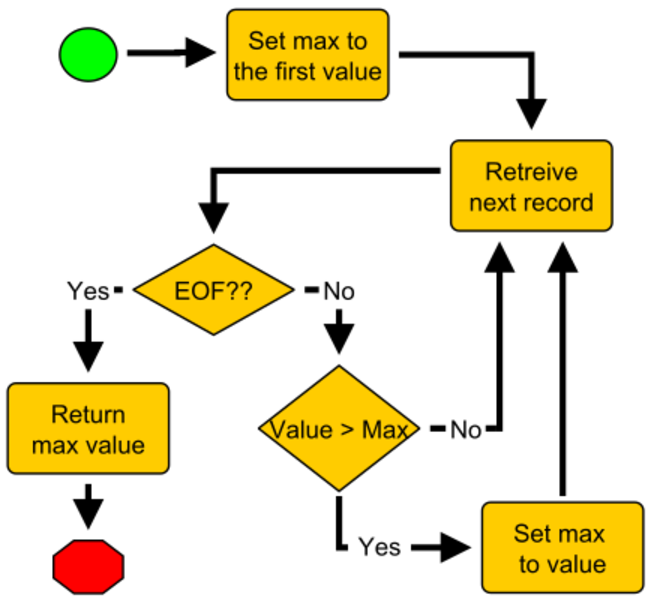
\includegraphics[width=0.8\columnwidth]{img/flowchart.pdf}
\caption{The Logic of the Max() Function}
\label{fig_flowchart}
\end{figure}

Figure~\ref{fig_doublecolumn} is an example of a double column floating figure that extends to the width of the page.

\begin{figure*}[!t]
\centering
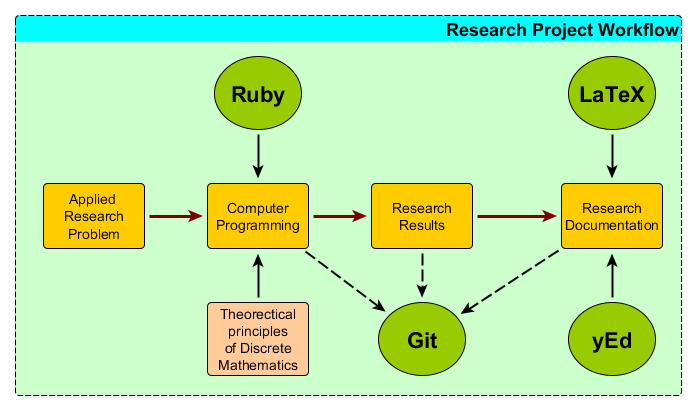
\includegraphics[width=\textwidth,height=3in]{img/researchprojectWork.png}%
\caption{Simulation results.}
\label{fig_doublecolumn}
\end{figure*}


\section{Methodology}

In this section describe your method to collect data for this research.

Normally a paper will be about 50-75\% text which will provide suitable padding between tables, equlations and illustrations. For this reason, these non-text objects are labeled and referenced so that the materials can be found even if the object is floated to subsequent pages.

The class logo is seen as a floating illustration in Figure~\ref{fig_classlogo}.

\begin{figure}[htb]
\centering
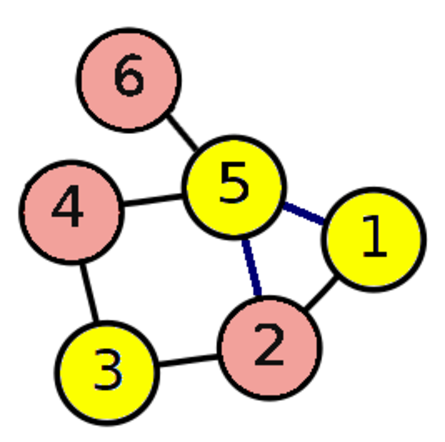
\includegraphics[width=0.5\columnwidth]{img/classlogo.pdf}
\caption{The class logo.}
\label{fig_classlogo}
\end{figure}

It is also good to include relevant mathematic formula. This is relatively easy to do as shown by the Taylor series for approximating the value of $e^x$ given in Equation~\ref{taylorseries}.

\begin{equation}
\label{taylorseries}
e^x = {x^0\over 0!} + {x^1\over 1!} + {x^2\over 2!} +{x^3\over 3!} + ...= \sum^\infty_{n=0}\ {x^n\over n!}
\end{equation}

Describe the programming environment and the approach used to collect data to address the research question being addressed.

\begin{equation}
\label{ts}
c=\sqrt{a^2+b^2 +D^2 + e^{2X}\over 2}
\end{equation}

Many parameters can be listed in a simple table as shown in  Table \ref{progenv}

\begin{table}[htb]
\centering
\caption{Programming environment}
\medskip
\label{progenv}
\begin{tabular}{lc}
\textbf{Parameter} & \textbf{Value}\\
CPU & Z80, 1 MHz\\
RAM Memory & 16 K\\
Ext Memory & 1 MB\\
Programming language & C \\
Communication& Bluetooth \\
\end{tabular}
\end{table}

Table~\ref{progenv} An example of a floating table. Note that, for IEEE style tables, the 
\verb|\caption| command should come BEFORE the table. Table text will default to
\verb|\footnotesize| as IEEE normally uses this smaller font for tables.
The \verb|\label| must come after \verb|\caption| as always.

Note that IEEE typically puts floats only at the top, even when this
results in a large percentage of a column being occupied by floats.

\section{Results}
\label{sec:results}

In this section provide a summary of the data collected. You can use graphs, and tables to represent your results.
Provide tables and graphs that summary of the information collected. Figure \ref{fig_experiment}
is a scatterplot of experimental data. 

\begin{figure}[htb]
\centering
\caption{Experimental data}
\label{fig_experiment}
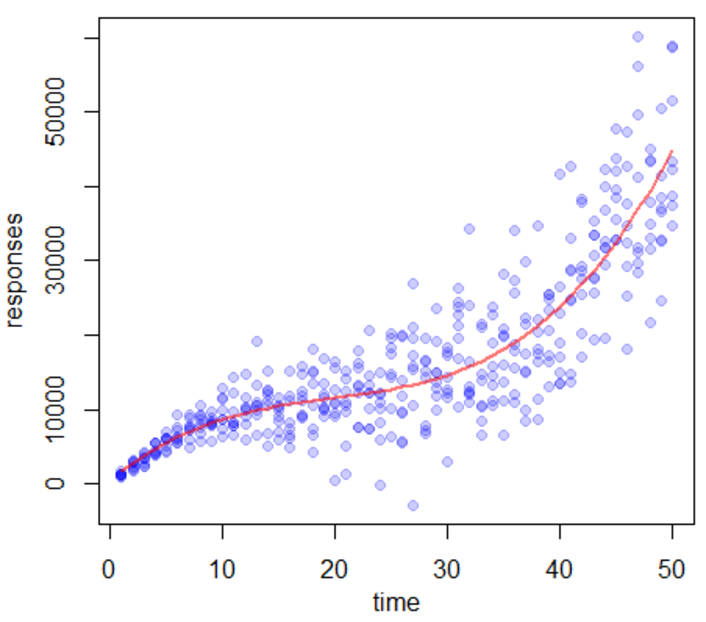
\includegraphics[width=0.9\columnwidth]{img/experiment.pdf}
\end{figure}

Floating figures will be placed in the next appropriate place. For example, Figure \ref{fig_histogram} is a histogram created in R.

\begin{figure}[htb]
\centering
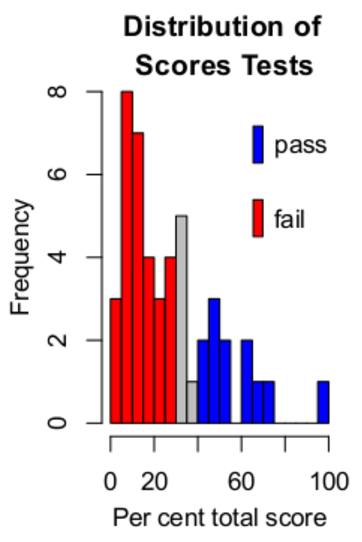
\includegraphics[width=0.8\columnwidth,height=2.5in]{img/Rplot.pdf}
\caption{Freshmen Math Grades}
\label{fig_histogram}
\end{figure}

\section{Discussion}
This section will interpret and discuss the findings presented in Section \ref{sec:results}

\begin{itemize}
\item Retrieval speed of data decreases linearly with the array size.
\item Energy consumption is proportional to the time required.
\item Search for elements within a sorted list decreases both the time and energy required for data retrieval.
\end{itemize}

The conclusion summarizes the results and suggest broader implications and applications of this information and methodology for real world problems.
The final paragraphs should suggest the following:
 
 \begin{itemize}
 \item implications of this research (Using indices make programs run faster and greener).
 \item a future direction for this research. (Further work is needed to determine the efficiency of different kinds of indices.)
\end{itemize}

\appendices
\section{Algorithm Used}

This will provide a simple diagram or psuedocode algorithm used for this research. Algorithm \ref{euclid} is one of the oldest recursive algorithms known to man. The idea is to recursively search for remainders.

\begin{algorithm}[htb]
    \caption{Euclid's Algorithm}
    \label{euclid}
    \begin{algorithmic}[1] % Line counting starts at 1
        \Procedure{Euclid}{$a,b$} \Comment {The GCD of a and b}
            \State $r\gets a \bmod b$
            \While{$r\not=0$} \Comment{Until rmdr is 0}
                \State $a \gets b$
                \State $b \gets r$
                \State $r \gets a \bmod b$
            \EndWhile\label{euclidendwhile}
            \State \textbf{return} $b$\Comment{The gcd is b}
        \EndProcedure
    \end{algorithmic}
\end{algorithm}

\section{Source Code}
Significant segments of the source code developed for this research can be listed here as shown in Listing~\ref{RubySetClass}. 

\begin{code}
\caption{Ruby Set Class Example3}
\label{RubySetClass}
\begin{lstlisting}[language=Ruby]
require 'set'
setA = Set.new(1..4)
setB = Set.new([2,3])

puts <<"ENDMSG"
  B subset A?: #{setB.subset?(setA)}
  A union B: #{setA.union(setB).inspect}
  A Not B: #{setA.subtract(setB).inspect}
ENDMSG
\end{lstlisting}
\end{code}

In this case two sets: $A$ and $B$ are created and manipulated according to standard set operations. This is provided as part of the basic Rudy language but does require an \verb|require| function to load the corresponding library.

% use unnumbered section* for acknowledgement
\section*{Acknowledgment}

The authors would to acknowledge IEEE for the use of this \LaTeXe\ template. The authors would like to thank their students for their feedback and insights gained while using this to create their papers. There is also a Thai version of this file that uses a unicode verson of this template.

%\IEEEtriggeratref{8}
% The "triggered" command can be changed if desired:
%\IEEEtriggercmd{\enlargethispage{-5in}}

% references section
\bibliography{classrefs}%

\par\vfill
\end{document}

